\documentclass[10pt,a4paper]{article}
\usepackage{placeins}
\usepackage[utf8]{inputenc}
\usepackage[ruled]{algorithm2e}
\usepackage{fullpage}
\usepackage{graphicx}
\usepackage{float}
\usepackage[portuguese]{babel}
\usepackage[]{amsmath}
\restylefloat{figure}

\usepackage[adobe-utopia]{mathdesign}
\usepackage[T1]{fontenc}

% \usepackage{mdframed}

\DeclareGraphicsExtensions{.jpg,.pdf}

\numberwithin{equation}{section}

\title{Trabalho Prático 2 - Montador}
\author{Victor Pires Diniz}

\begin{document}
\maketitle
\begin{center}
Software Básico - 2º Semestre de 2015
\end{center}

\section{Descrição do trabalho}

O segundo trabalho prático do semestre envolve o desenvolvimento de um montador para o código de montagem de uma máquina virtual especificada, para a qual foi feito um emulador no trabalho prévio. Esse montador teria suporte a processamento de \emph{labels} para determinar posições de memória e também a algumas pseudo-instruções, além das vinte e duas instruções da máquina virtual. Com código de montagem, desenvolver programas para o emulador se torna muito mais simples, visto que o mesmo é de muito mais alto nível do que o código em linguagem de máquina, devido aos nomes mnemônicos, à presença das \emph{labels} e à possibilidade de uso de comentários.

\section{Implementação e decisões de projeto}

O código do montador está dividido semanticamente entre vários módulos:

\begin{itemize}
    \item \emph{main.c}: recebe parâmetros por linha de comando e chama o montador apropriadamente.
    \item Map (\emph{map.c, map.h, bucket.c, bucket.h}): implementa uma tabela de dispersão genérica, instanciada na tabela de símbolos e, também, na IDT.
    \item IDT (\emph{idt.c, idt.h}): implementa uma tabela que relaciona o nome das instruções às suas características e ao procedimento relacionado às pseudo-instruções.
    \item Pseudo-instruções (\emph{pseudo\_instr.c, pseudo\_instr.h}): contém dados sobre as pseudo-instruções, assim como funções que desempenham as ações associadas a elas.
    \item Metadados das instruções reais (\emph{real\_md.c, real\_md.h}): contém vetores com metadados sobre cada instrução real, como, por exemplo, o número de operandos e o tipo de cada um deles.
    \item Função hash auxiliar (\emph{hash\_aux.c, hash\_aux.h}): contém uma função para hashing de string.
    \item Montador (\emph{assembler.c, assembler.h}): implementa o montador e os procedimentos relacionados a ele.
\end{itemize}

Os mais importantes deles serão analisados a seguir em mais detalhe.

\subsection{Map}

O módulo map contém a implementação de uma hash table totalmente genérica, com tratamento de colisão através de listas encadeadas, definidas nos arquivos \emph{bucket.c} e \emph{bucket.h}. A interface para o tipo contém, entre outras funcionalidades, um pseudo-iterador, que é utilizado na impressão da tabela de símbolos em modo verboso.

\subsection{IDT}

Esse módulo cria uma \emph{instruction data table}, que relaciona o nome de cada instrução ou pseudo-instrução aos dados necessários para sua montagem (ou execução, no caso das pseudo-instruções). Para isso, são utilizados dados sobre essas instruções, disponíveis nos módulos \emph{pseudo\_instr} e \emph{real\_md}. A função \emph{idtCreate} gera uma hash table indexada por strings, cujos valores são estruturas que contém um tipo \emph{PseudoInstr} ou \emph{RealMD}, a depender de se tratar de uma instrução real ou não.

\subsubsection{Montador}

O montador opera em dois passos principais. Ambos mantém o estado do montador através do \emph{instruction location counter} (ILC), incrementado na leitura de cada operador ou operando. Além disso, eles compartilham o uso da função \emph{asmParseLine}, que divide cada linha em seus componentes: \emph{label}, \emph{operador} e dois possíveis operandos.

O primeiro deles, desempenhado na função \emph{asmBuildSymTable}, consiste em passar pelo código de montagem em busca de labels, registrando a posição de cada uma (de acordo com o ILC) na tabela de símbolos. Outras funções associadas à tabela de símbolos são \emph{asmDestroySymTable} e \emph{asmPrintSymTable}, que liberam a memória associada à tabela e a imprimem, respectivamente.

Ao passar pela segunda vez, com a função \emph{asmReplaceAndSave}, a montagem real é realizada, imprimindo para o arquivo de saída o código de máquina associado a cada instrução. Nessa fase, as labels são substituídas pelo endereço presente na tabela de símbolos, com compensação relativa ao ILC atual, para garantir que os endereços sejam utilizados relativamente ao contador de programa, como proposto na especificação da máquina. A função \emph{assembleOperand} é utilizada para imprimir diferentemente operandos registradores ou valores imediatos, visto que é necessário tratá-los de formas diferentes.

\section{Compilação e execução}

A compilação do montador pode ser realizada através da \emph{makefile} disponibilizada ou diretamente através do \emph{GCC} ou outro compilador C. Caso compilado através da \emph{makefile}, o executável estará localizado na pasta \verb|bin/|. A execução do programa deve ser realizada através da linha de comando, na seguinte forma,

\begin{verbatim}
    {endereço do executável do montador} <input_addr> <output_addr> [output_mode]
\end{verbatim}

em que:

\begin{itemize}
    \item \verb|input_addr|: endereço para o arquivo de entrada, em código de montagem.
    \item \verb|output_addr|: endereço para o arquivo de saída a ser criado.
    \item \verb|output_mode|: parâmetro \textbf{opcional} que permite escolher entre os modos de execução simples e verboso. Caso não seja especificado, o programa é executado em modo simples, sem informação de depuração. Valores válidos: \verb|s| (simples) ou \verb|v| (verboso).
\end{itemize}

\section{Testes realizados}

Na pasta de testes presente no pacote deste trabalho, há diversos programas que foram utilizados para garantir o bom funcionamento do montador, cobrindo todas as instruções disponibilizadas pela especificação da máquina virtual. Vários deles foram implementados de acordo com o pedido na especificação do trabalho. Imagens da execução dos testes estão disponíveis no apêndice desta documentação. Segue abaixo uma breve descrição do comportamento de cada programa:

\begin{itemize}
    \item \verb|tspec.i|: teste disponibilizado na especificação do trabalho. Determina o maior número entre dois valores informados.
    \item \verb|tfib.i|: calcula o número de Fibonacci de acordo com um índice fornecido pelo usuário. (Requerido na especificação.)
    \item \verb|texp.i|: realiza a exponenciação de um número, de acordo com uma base e um expoente, ambos fornecidos pelo usuário. (Requerido na especificação.)
    \item \verb|tdiv.i|: realiza a divisão por força bruta de dois números inteiros, retornando quociente e resto. (Requerido na especificação.)
    \item \verb|tmdn.i|: determina a mediana de um conjunto de sete itens fornecidos pelo usuário. (Requerido na especificação.)
    \item \verb|tothers.i|: realiza operações variadas com instruções que não foram cobertas pelos outros testes, para garantir o bom funcionamento de tudo.
\end{itemize}

\subsection{Testes unitários}

Além das entradas de teste elaboradas, foram criados também diversos \emph{unit tests}, com o propósito de testar a funcionalidade de cada módulo do montador. Esses testes estão disponíveis na pasta \verb|unit-tests/|, dentro da pasta de testes, e podem ser compilados com o comando \verb|make tests|, que utiliza uma funcionalidade adicional da \emph{makefile} providenciada. Após a compilação, eles estarão localizados na pasta \verb|bin/test-bin/|.

\section{Conclusão}

Neste trabalho, foi implementado um montador para uma máquina virtual, definido de acordo com a especificação fornecida. O comportamento e a implementação do montador foram discutidos no contexto dos testes realizados e da interação com o emulador criado no trabalho prático anterior, de forma a garantir que as instruções e pseudo-instruções funcionam como previsto.

\appendix

\section{Imagens de execução dos testes}

\begin{figure}[h]
    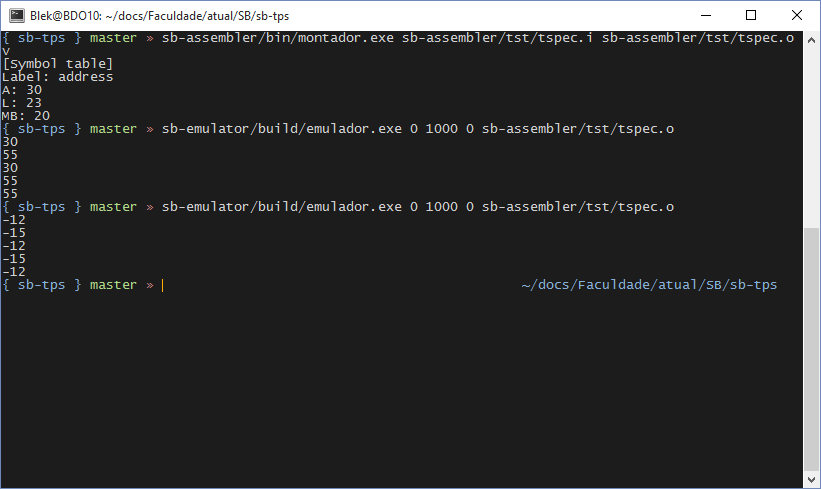
\includegraphics[scale=0.7]{imagens/tspec_console.png}
    \centering
    \caption{Montagem em modo verboso e execução do teste tspec.i.}
\end{figure}

\begin{figure}[h]
    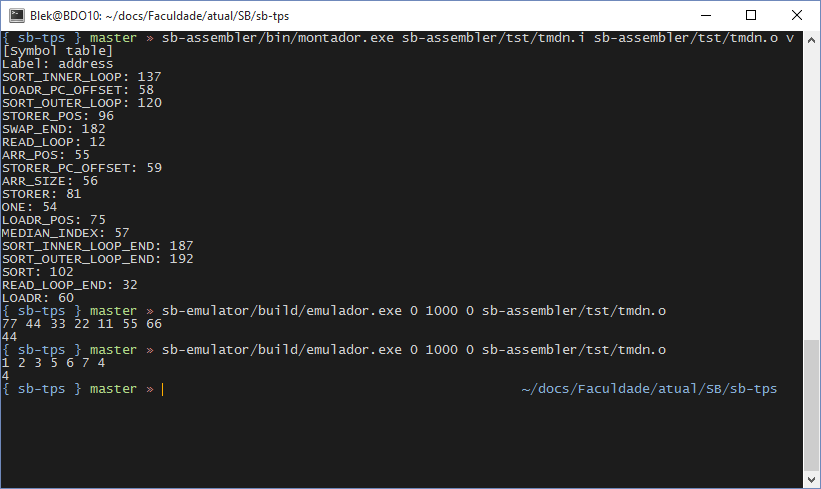
\includegraphics[scale=0.7]{imagens/tmdn_console.png}
    \centering
    \caption{Montagem em modo verboso e execução do teste tmdn.i.}
\end{figure}

\begin{figure}[h]
    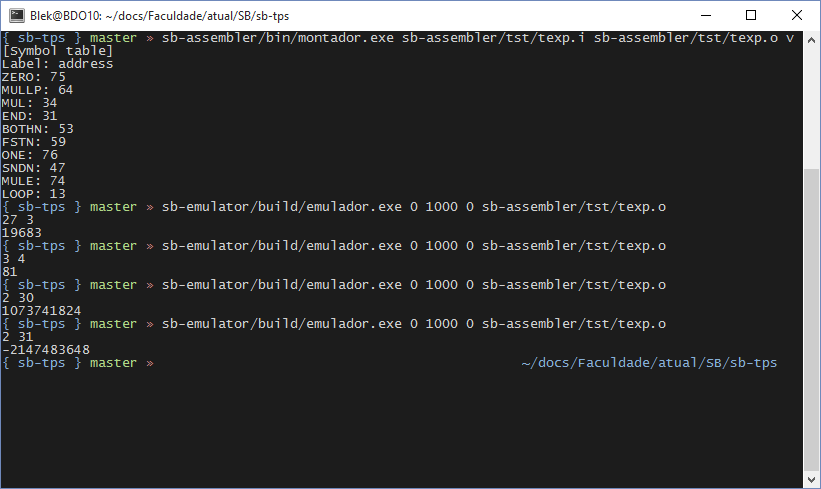
\includegraphics[scale=0.7]{imagens/texp_console.png}
    \centering
    \caption{Montagem em modo verboso e execução do teste texp.i.}
\end{figure}

\begin{figure}[h]
    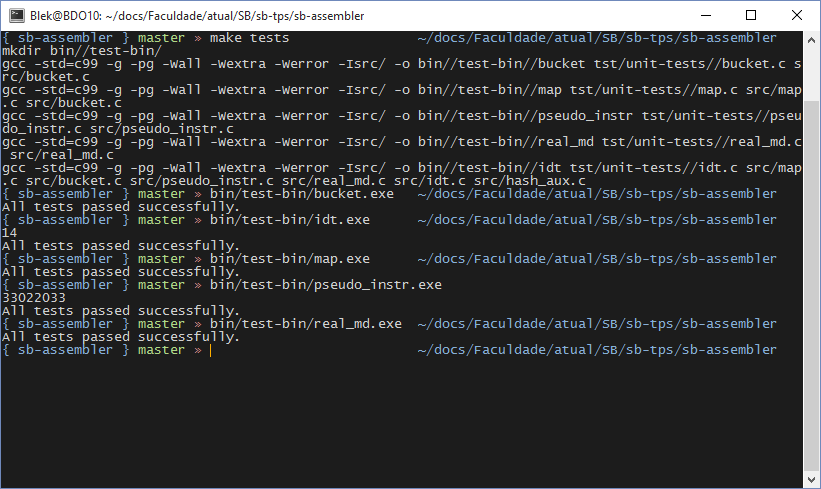
\includegraphics[scale=0.7]{imagens/unit_tests_console.png}
    \centering
    \caption{Compilação e execução dos testes unitários providenciados.}
\end{figure}

\FloatBarrier

\end{document}